\section{Color planes}
\begin{enumerate}[label=\emph{\alph*)}]
\item Swap the red and blue channels of the input image.

The results are shown in figure \ref{fig:swap-channel}. The $imread()$ instruction of OpenCV reads images in format BGR, then we have to swap the channel blue(first channel) with the channel red(third channel), generating a new image in RGB format.

\begin{figure}[h!]
\centering
\begin{subfigure}{0.5\textwidth}
  \centering
  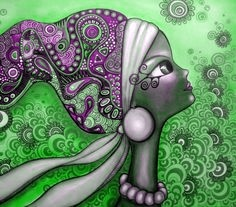
\includegraphics[width=0.5\linewidth]{../output/p0-2-a-0.jpg}
  \caption{Output for the input p0-1-0.jpg}
  \label{fig:sfig1}
\end{subfigure}%
\begin{subfigure}{0.5\textwidth}
  \centering
  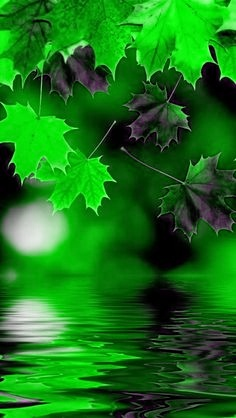
\includegraphics[width=0.5\linewidth]{../output/p0-2-a-1.jpg}
  \caption{Output for the input p0-1-1.jpg}
  \label{fig:sfig2}
\end{subfigure}
\begin{subfigure}{0.5\textwidth}
  \centering
  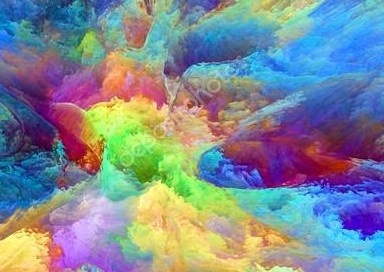
\includegraphics[width=0.5\linewidth]{../output/p0-2-a-2.jpg}
  \caption{Output for the input p0-1-2.jpg}
  \label{fig:sfig1}
\end{subfigure}%
\begin{subfigure}{0.5\textwidth}
  \centering
  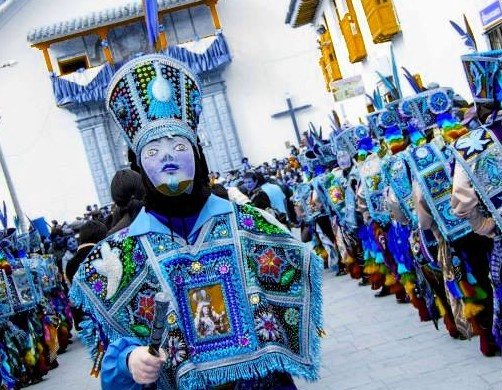
\includegraphics[width=0.5\linewidth]{../output/p0-2-a-3.jpg}
  \caption{Output for the input p0-1-3.jpg}
  \label{fig:sfig2}
\end{subfigure}
\caption{Output images for question 2.a}
\label{fig:swap-channel}
\end{figure}

\item Create a monochrome image (img-green) by selecting the green channel of the input image.

The results are shown in figure \ref{fig:green-channel}. As we extract the green channel from the original image to generate a monochromatic image, then, the regions of the image that depend more on green color will have values close to 255 in the channel green, which means that in the output image those regions will have a color close to white, while the other regions of the image will have a color close to black.\\

\begin{figure}[h!]
\centering
\begin{subfigure}{0.5\textwidth}
  \centering
  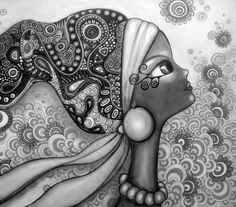
\includegraphics[width=0.5\linewidth]{../output/p0-2-b-0.jpg}
  \caption{Output for the input p0-1-0.jpg}
  \label{fig:sfig1}
\end{subfigure}%
\begin{subfigure}{0.5\textwidth}
  \centering
  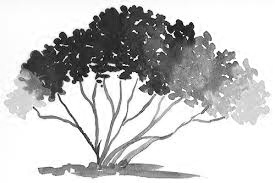
\includegraphics[width=0.5\linewidth]{../output/p0-2-b-1.jpg}
  \caption{Output for the input p0-1-1.jpg}
  \label{fig:sfig2}
\end{subfigure}
\begin{subfigure}{0.5\textwidth}
  \centering
  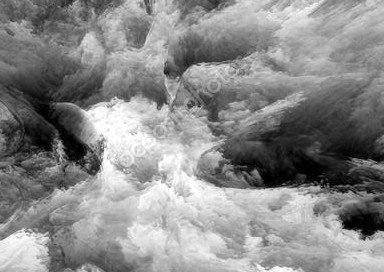
\includegraphics[width=0.5\linewidth]{../output/p0-2-b-2.jpg}
  \caption{Output for the input p0-1-2.jpg}
  \label{fig:sfig1}
\end{subfigure}%
\begin{subfigure}{0.5\textwidth}
  \centering
  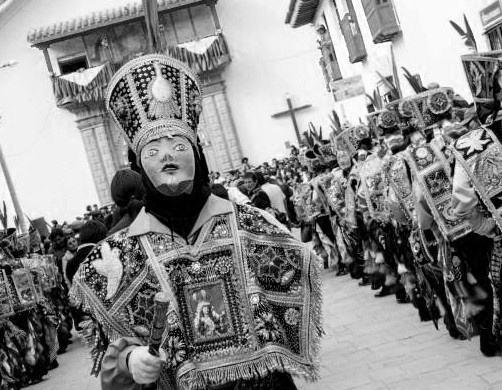
\includegraphics[width=0.5\linewidth]{../output/p0-2-b-3.jpg}
  \caption{Output for the input p0-1-3.jpg}
  \label{fig:sfig2}
\end{subfigure}
\caption{Output images for question 2.b}
\label{fig:green-channel}
\end{figure}

\item Create a monochrome image (img-red) by selecting the red channel of the first input image.

The results are shown in figure \ref{fig:red-channel}. Similar to the previous interpretation, we say that the light colored regions in the output image  corresponds to regions with high red values in the original image.
\begin{figure}[h!]
\centering
\begin{subfigure}{0.5\textwidth}
  \centering
  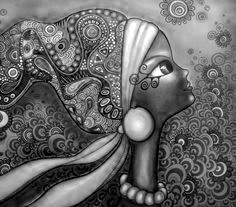
\includegraphics[width=0.5\linewidth]{../output/p0-2-c-0.jpg}
  \caption{Figura 13. Output for the input p0-1-0.jpg}
  \label{fig:sfig1}
\end{subfigure}%
\begin{subfigure}{0.5\textwidth}
  \centering
  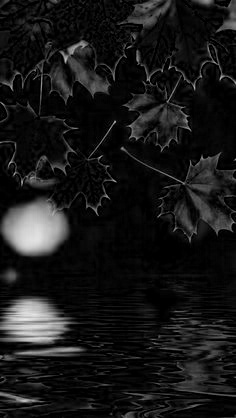
\includegraphics[width=0.5\linewidth]{../output/p0-2-c-1.jpg}
  \caption{Figura 14. Output for the input p0-1-1.jpg}
  \label{fig:sfig2}
\end{subfigure}
\begin{subfigure}{0.5\textwidth}
  \centering
  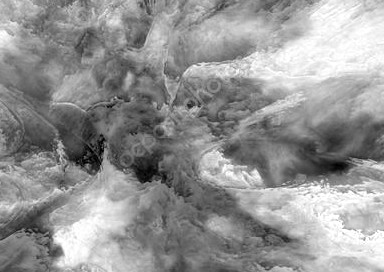
\includegraphics[width=0.5\linewidth]{../output/p0-2-c-2.jpg}
  \caption{Figura 15. Output for the input p0-1-0.jpg}
  \label{fig:sfig1}
\end{subfigure}%
\begin{subfigure}{0.5\textwidth}
  \centering
  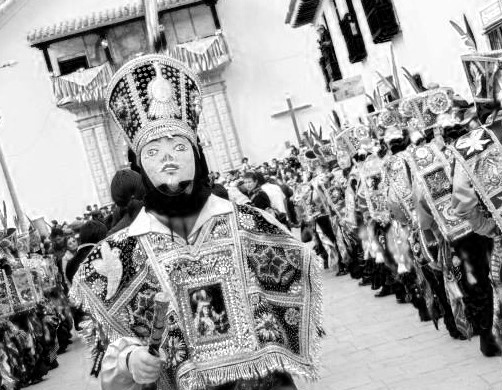
\includegraphics[width=0.5\linewidth]{../output/p0-2-c-3.jpg}
  \caption{Figura 16. Output for the input p0-1-1.jpg}
  \label{fig:sfig2}
\end{subfigure}
\caption{Output images for question 2.c}
\label{fig:red-channel}
\end{figure}

\item Which image looks more like what you would expect a monochrome image to look like? Would you expect a computer vision algorithm to work on one better than the other? Why?

The monochrome image generated from the green channel most closely resembles the monochrome image. The intuition behind this effect is that in one of the popular formulas to convert $RGB$ to grayscale images ($R \times 0.29 + G \times 0,58 + B \times 0,11$) the green channel has bigger weighting. 

A Computer Vision algorithm would work better in one representation, depending of the image properties, e.g. suppose that we have an image that has lower values in the red channel, thus using a monochromatic representation using this channel has a lot of black areas and this may yield in a worse results. On the hand, using the green channel would make the image more discriminative. Analogously, the same would occurs with an image with low green values.


\end{enumerate}
